% needed packages:
% \usetikzlibrary{patterns}


\newcommand{\Perceptron}{
  \begin{center}
  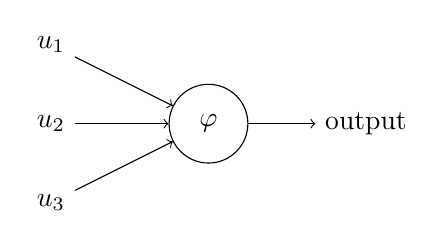
\begin{tikzpicture}[scale=1]

    \node[circle, draw, minimum size=1cm] at (0,0) (act) {$\varphi$};
    \node at (-2,  1) (u1) {$u_1$};
    \node at (-2, -0) (u2) {$u_2$};
    \node at (-2, -1) (u3) {$u_3$};
    \node at ( 2,  0) (out) {output};

    \path[draw, ->] (u1) edge (act) node {};
    \path[draw, ->] (u2) edge (act) node {};
    \path[draw, ->] (u3) edge (act) node {};
    \path[draw, ->] (act) edge (out) node {};

  \end{tikzpicture}
  \end{center}
}

\newcommand{\FeedForwardNet}[1]{
  \begin{center}
  \begin{tikzpicture}[scale=#1]
    \node[circle, draw, scale=#1] at (-1.5,0) (11) {};
    \node[circle, draw, scale=#1] at (-1.5,1) (12) {};
    \node[circle, draw, scale=#1] at (-1.5,2) (13) {};

    \foreach \n in {21, ..., 28}{
      \node[circle, draw, scale=#1] at (0, \n*.4 - 22*.4) (\n) {};
    }

    \foreach \idx in {11,...,13} {
      \foreach \jdx in {21,...,28} {
        \path[draw, ->] (\idx) edge (\jdx) node {};
      }
    }

    \node[circle, draw, scale=#1] at (1.5, 0.5) (31) {};
    \node[circle, draw, scale=#1] at (1.5, 1.5) (32) {};

    \foreach \idx in {21,...,28} {
      \foreach \jdx in {31,...,32} {
        \path[draw, ->] (\idx) edge (\jdx) node {};
      }
    }
  \end{tikzpicture}
  \end{center}
}

\newcommand{\RecurrentNet}{
  \begin{center}
  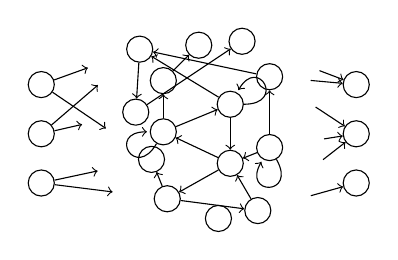
\begin{tikzpicture}[scale=.5]
    % input nodes
    \node[circle, draw] at (-1,1.5) (11) {};
    \node[circle, draw] at (-1,2.75) (12) {};
    \node[circle, draw] at (-1,4) (13) {};
    % reservoir nodes
    \node[circle, draw] at (2.2,1.1) (21) {};
    \node[circle, draw] at (4.5,0.8) (22) {};
    \node[circle, draw] at (4.8,2.4) (23) {};
    \node[circle, draw] at (1.4,3.3) (24) {};
    \node[circle, draw] at (2.1,2.8) (25) {};
    \node[circle, draw] at (3.8,3.5) (26) {};
    \node[circle, draw] at (4.8,4.2) (27) {};
    \node[circle, draw] at (1.5,4.9) (28) {};
    \node[circle, draw] at (2.1,4.1) (29) {};
    \node[circle, draw] at (3.8,2.0) (30) {};
    \node[circle, draw] at (3.5,0.6) (31) {};
    \node[circle, draw] at (3.0,5.0) (32) {};
    \node[circle, draw] at (4.1,5.1) (33) {};
    \node[circle, draw] at (1.8,2.1) (34) {};
    % output nodes
    \node[circle, draw] at (7,1.5)  (41) {};
    \node[circle, draw] at (7,2.75) (42) {};
    \node[circle, draw] at (7,4)    (43) {};

    % input connections
    \path[shorten >= 15pt, draw, ->] (12) edge (24) node {};
    \path[shorten >= 15pt, draw, ->] (12) edge (28) node {};
    \path[shorten >= 15pt, draw, ->] (11) edge (34) node {};
    \path[shorten >= 15pt, draw, ->] (11) edge (21) node {};
    \path[shorten >= 15pt, draw, ->] (13) edge (34) node {};
    \path[shorten >= 15pt, draw, ->] (13) edge (28) node {};
    % reservoir connections
    \path[draw, ->] (21) edge (22) node {};
    \path[draw, ->] (21) edge (34) node {};
    \path[draw, ->] (22) edge (30) node {};
    \path[draw, ->] (23) edge (30) node {};
    \path[draw, ->] (23) edge (27) node {};
    \path[draw, ->] (23) edge[in=-120, out=-60, loop] (23) node {};
    \path[draw, ->] (24) edge (33) node {};
    \path[draw, ->] (25) edge (26) node {};
    \path[draw, ->] (25) edge[in=-180, out=-120, loop] (25) node {};
    \path[draw, ->] (25) edge (29) node {};
    \path[draw, ->] (26) edge (28) node {};
    \path[draw, ->] (26) edge (30) node {};
    \path[draw, ->] (26) edge[in=60, out=0, loop] (26) node {};
    \path[draw, ->] (27) edge (28) node {};
    \path[draw, ->] (28) edge (24) node {};
    \path[draw, ->] (29) edge (32) node {};
    \path[draw, ->] (30) edge (25) node {};
    \path[draw, ->] (30) edge (21) node {};
    % output connections
    \path[shorten <= 10pt, draw, ->] (27) edge (43) node {};
    \path[shorten <= 15pt, draw, ->] (27) edge (42) node {};
    \path[shorten <= 15pt, draw, ->] (23) edge (42) node {};
    \path[shorten <= 15pt, draw, ->] (22) edge (41) node {};
    \path[shorten <= 25pt, draw, ->] (22) edge (42) node {};
    \path[shorten <= 25pt, draw, ->] (33) edge (43) node {};
    % output feedback paths
    %\draw[->] (41) -- (8.3, 1.5) -- (8.3, 6.7) -- (-2.3, 6.7) -- (-2.3, 1.5) -- (11);
    %\draw[->] (42) -- (8.1, 2.75) -- (8.1, 6.5) -- (-2.1, 6.5) -- (-2.1, 2.75) -- (12);
    %\draw[->] (43) -- (7.9, 4) -- (7.9, 6.3) -- (-1.9, 6.3) -- (-1.9, 4) -- (13);


  \end{tikzpicture}
  \end{center}
}

\newcommand{\RecurrentNetAnnotated}{
  \begin{center}
  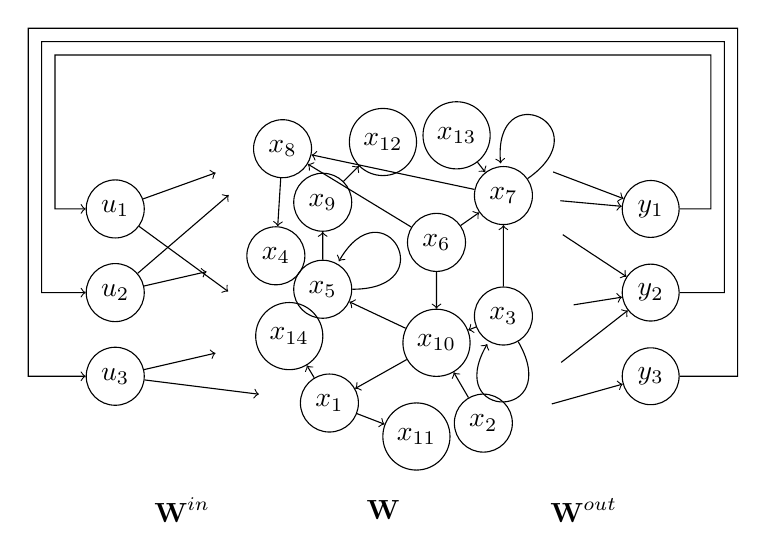
\begin{tikzpicture}[scale=.85]
    % annotations
    \node at ( 0, -0.5) (win) {$\textbf{W}^{\text{in}}$};
    \node at ( 3, -0.5) (w) {$\textbf{W}$};
   \node at ( 6, -0.5) (wout) {$\textbf{W}^{\text{out}}$};

    % input nodes
    \node[circle, draw] at (-1,1.5) (11)  {$u_{3}$};
    \node[circle, draw] at (-1,2.75) (12) {$u_{2}$};
    \node[circle, draw] at (-1,4) (13)    {$u_{1}$};
    % reservoir nodes
    \node[circle, draw] at (2.2,1.1) (21) {$x_{1}$};
    \node[circle, draw] at (4.5,0.8) (22) {$x_{2}$};
    \node[circle, draw] at (4.8,2.4) (23) {$x_{3}$};
    \node[circle, draw] at (1.4,3.3) (24) {$x_{4}$};
    \node[circle, draw] at (2.1,2.8) (25) {$x_{5}$};
    \node[circle, draw] at (3.8,3.5) (26) {$x_{6}$};
    \node[circle, draw] at (4.8,4.2) (27) {$x_{7}$};
    \node[circle, draw] at (1.5,4.9) (28) {$x_{8}$};
    \node[circle, draw] at (2.1,4.1) (29) {$x_{9}$};
    \node[circle, draw] at (3.8,2.0) (30) {$x_{10}$};
    \node[circle, draw] at (3.5,0.6) (31) {$x_{11}$};
    \node[circle, draw] at (3.0,5.0) (32) {$x_{12}$};
    \node[circle, draw] at (4.1,5.1) (33) {$x_{13}$};
    \node[circle, draw] at (1.6,2.1) (34) {$x_{14}$};
    % output nodes
    \node[circle, draw] at (7,1.5)  (41) {$y_{3}$};
    \node[circle, draw] at (7,2.75) (42) {$y_{2}$};
    \node[circle, draw] at (7,4)    (43) {$y_{1}$};

    % input connections
    \path[shorten >= 15pt, draw, ->] (12) edge (24) node {};
    \path[shorten >= 15pt, draw, ->] (12) edge (28) node {};
    \path[shorten >= 15pt, draw, ->] (11) edge (34) node {};
    \path[shorten >= 15pt, draw, ->] (11) edge (21) node {};
    \path[shorten >= 15pt, draw, ->] (13) edge (34) node {};
    \path[shorten >= 15pt, draw, ->] (13) edge (28) node {};
    % reservoir connections
    \path[draw, ->] (21) edge (31) node {};
    \path[draw, ->] (21) edge (34) node {};
    \path[draw, ->] (22) edge (30) node {};
    \path[draw, ->] (23) edge (30) node {};
    \path[draw, ->] (23) edge (27) node {};
    \path[draw, ->] (23) edge[in=-120, out=-60, loop] (23) node {};
    \path[draw, ->] (25) edge[in=60, out=0, loop] (25) node {};
    \path[draw, ->] (25) edge (29) node {};
    \path[draw, ->] (26) edge (28) node {};
    \path[draw, ->] (26) edge (30) node {};
    \path[draw, ->] (26) edge (27) node {};
    \path[draw, ->] (27) edge[in=95, out=35, loop] (27) node {};
    \path[draw, ->] (27) edge (28) node {};
    \path[draw, ->] (28) edge (24) node {};
    \path[draw, ->] (29) edge (32) node {};
    \path[draw, ->] (30) edge (25) node {};
    \path[draw, ->] (30) edge (21) node {};
    \path[draw, ->] (33) edge (27) node {};
    % output connections
    \path[shorten <= 10pt, draw, ->] (27) edge (43) node {};
    \path[shorten <= 15pt, draw, ->] (27) edge (42) node {};
    \path[shorten <= 15pt, draw, ->] (23) edge (42) node {};
    \path[shorten <= 15pt, draw, ->] (22) edge (41) node {};
    \path[shorten <= 25pt, draw, ->] (22) edge (42) node {};
    \path[shorten <= 25pt, draw, ->] (33) edge (43) node {};

    % output feedback paths
    \draw[->] (41) -- (8.3, 1.5) -- (8.3, 6.7) -- (-2.3, 6.7) -- (-2.3, 1.5) -- (11);
    \draw[->] (42) -- (8.1, 2.75) -- (8.1, 6.5) -- (-2.1, 6.5) -- (-2.1, 2.75) -- (12);
    \draw[->] (43) -- (7.9, 4) -- (7.9, 6.3) -- (-1.9, 6.3) -- (-1.9, 4) -- (13);

    %\draw[->] (7.9, 2.75) -- (8.5, 2.75) -- (8.5, 6.5)
    %  -- (-2.5, 6.5) -- (-2.5, 2.75) -- (-1.9, 2.75);
    %\draw (7.9, 1.2) -- (7.9, 4.3);
    %\draw (-1.9, 1.2) -- (-1.9, 4.3);

  \end{tikzpicture}
  \end{center}
}

\newcommand{\RNNFlowChart}{
  \begin{center}
  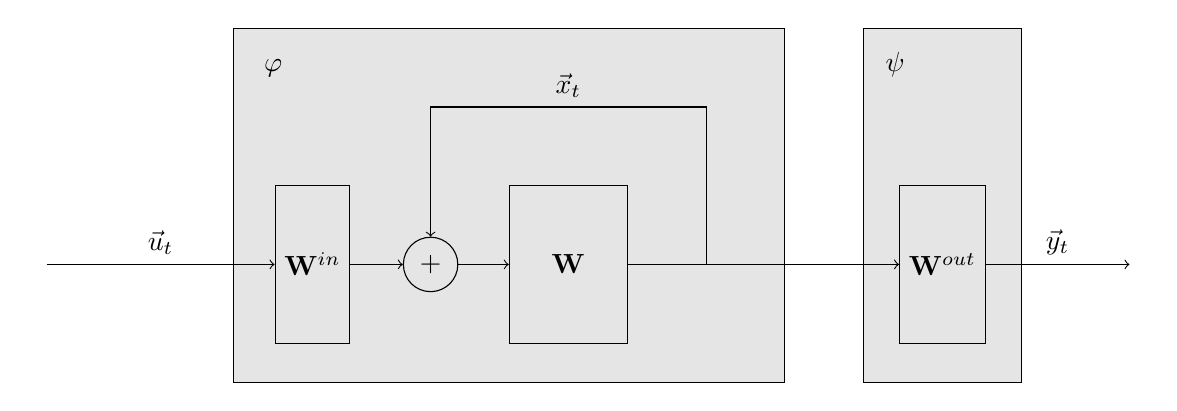
\begin{tikzpicture}[scale=1]
    \node[draw, rectangle,
          minimum width=7cm, minimum height=4.5cm,
          label={[shift={(-3,-.75)}]$\varphi$},
          fill=black!10,
          ] (Phi) at (4.5, 0.75) {};

    \node[draw, rectangle,
          minimum width=2cm, minimum height=4.5cm,
          label={[shift={(-.6,-.75)}]$\psi$},
          fill=black!10,
          ] (Psi) at (10, 0.75) {};

    \node (ut) at (-1.5,0) {};
    \node[draw, rectangle, minimum height=2cm]
        (Win) at (2,0) {$\mathbf{W}^{\text{in}}$};
    \node[draw, circle] (u+x) at (3.5,0) {+};
    \node[draw, rectangle, minimum height=2cm, minimum width=1.5cm]
        (W) at (5.25, 0) {$\mathbf{W}$};
    \node[draw, rectangle, minimum height=2cm] 
        (Wout) at (10,0) {$\mathbf{W}^{\text{out}}$};
    \node (yt) at (12.5, 0) {};

    \path[draw, ->] (ut) edge node[above] {$\vec{u}_t$} (Win);
    \path[draw, ->] (Win) edge (u+x) {};
    \path[draw, ->] (u+x) edge (W) {};
    \path[draw, ->] (W) edge (Wout) {};

    \path[draw, ->] (7, 0) -- (7, 2) 
        -- (5.25, 2) node[above] {$\vec{x}_t$} -- (3.5, 2) -- (u+x);
    \path[draw, ->] (Wout) edge node[above] {$\vec{y}_t$} (yt);
  \end{tikzpicture}
  \end{center}
}

\newcommand{\ESNFlowChart}{
  \begin{center}
  \begin{tikzpicture}[scale=1]
    \node[draw, rectangle,
          minimum width=7cm, minimum height=4.5cm,
          label={[shift={(-3,-.75)}]$\varphi$},
          fill=black!10,
          ] (Phi) at (4.5, 0.75) {};

    \node[draw, rectangle,
          minimum width=2cm, minimum height=4.5cm,
          label={[shift={(-.6,-.75)}]$\psi$},
          fill=black!10,
          ] (Psi) at (10, 0.75) {};

    \node (ut) at (-1.5,0) {};
    \node[draw, rectangle, minimum height=2cm,
          pattern=north west lines, pattern color=gray,
        ] (Win) at (2,0) {$\mathbf{W}^{\text{in}}$};
    \node[draw, circle] (u+x) at (3.5,0) {+};
    \node[draw, rectangle, minimum height=2cm, minimum width=1.5cm,
          pattern=north west lines, pattern color=gray,
        ] (W) at (5.25, 0) {$\mathbf{W}$};
    \node[draw, rectangle, minimum height=2cm] 
        (Wout) at (10,0) {$\mathbf{W}^{\text{out}}$};
    \node (yt) at (12.5, 0) {};

    \path[draw, ->] (ut) edge node[above] {$\vec{u}_t$} (Win);
    \path[draw, ->] (Win) edge (u+x) {};
    \path[draw, ->] (u+x) edge (W) {};
    \path[draw, ->] (W) edge (Wout) {};

    \path[draw, ->] (7, 0) -- (7, 2) 
        -- (5.25, 2) node[above] {$\vec{x}_t$} -- (3.5, 2) -- (u+x);
    \path[draw, ->] (Wout) edge node[above] {$\vec{y}_t$} (yt);
  \end{tikzpicture}
  \end{center}
}
